\section{Пространственная демонстрация результатов}

\subsection{Назначение пространственной демонстрации}

Следующим шагом после анализа отдельных примеров становится пространственная демонстрация результатов. Её задача
состоит в том, чтобы связать результаты рекомендательного и интерпретационного слоёв с конкретными полями и показать
возможный сценарий визуального анализа в пользовательском интерфейсе.

Для этого были подготовлены интерактивные карты и сводные таблицы, позволяющие сопоставлять положение полей,
рекомендации и интерпретационный контекст. Эти материалы показывают, как можно перейти от общего пространственного
контекста к анализу конкретного поля. В итоговом варианте карта связывает три типа информации:

\begin{itemize}
\tightlist
\item
  геометрическое или пространственное представление поля;
\item
  результат рекомендательного слоя для этого поля;
\item
  интерпретационный контекст для выбранного случая.
\end{itemize}

Иными словами, пространственная демонстрация переводит результат из формата таблиц и локальных графов в более
прикладной сценарий визуального анализа.

\subsection{Выбор локальной области на карте}

Для пространственной демонстрации используется выбор локальной области на карте. Пользователь задаёт прямоугольную
область интереса, после чего система отбирает поля, расположенные внутри неё.

Выбранная область используется как пространственный фильтр. Система показывает поля, попавшие внутрь неё, и тем самым
делает карту удобным средством перехода от общего обзора к локальному анализу.
В демонстрации акцент сделан на локальном сценарии: выборе области, просмотре полей внутри неё и переходе к рекомендациям
для конкретных участков.

\begin{figure}[H]
    \centering
    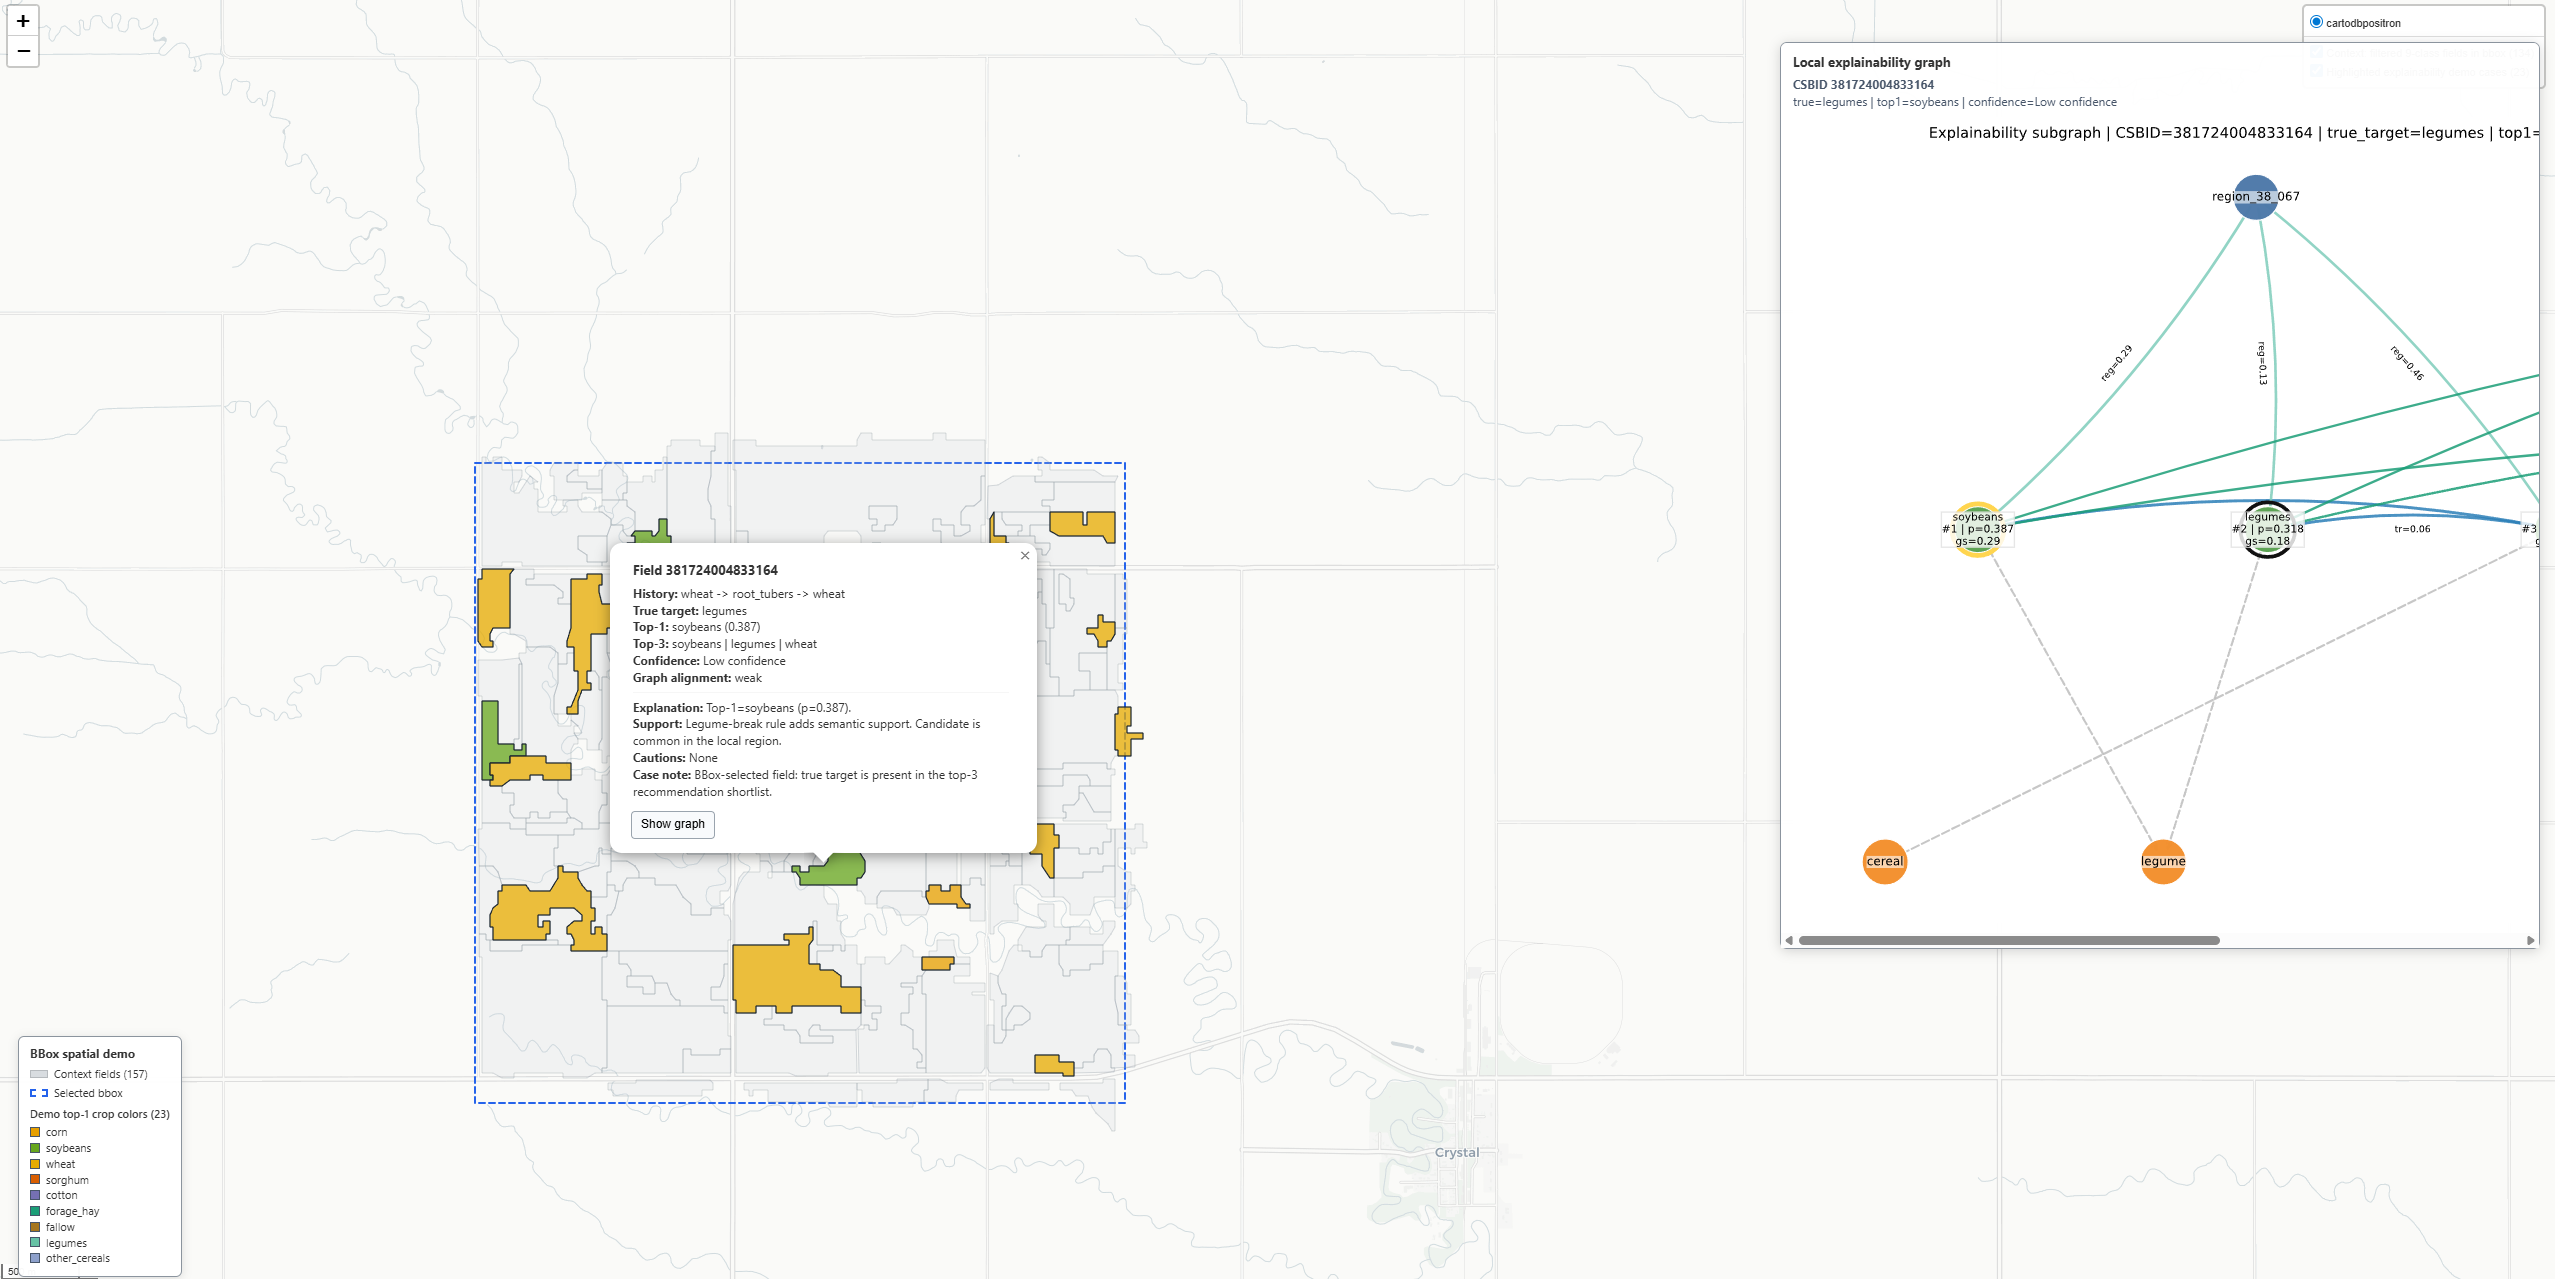
\includegraphics[width=0.95\textwidth]{figures/example_map.png}
    \caption{Пример пространственной демонстрации рекомендаций для выбранной локальной области}
    \label{fig:spatial-demo-map}
\end{figure}

На рисунке~\ref{fig:spatial-demo-map} показан пример выбранной локальной области. Пользователь может сначала определить
интересующий участок на карте, затем рассмотреть поля внутри него и перейти к анализу рекомендаций для отдельных объектов.

\subsection{Анализ полей внутри выбранной области}

После выбора области карта становится точкой входа в разбор конкретных полей. Для объектов, попавших внутрь выбранного
участка, могут быть показаны результаты рекомендательного слоя, уровень уверенности и интерпретационный контекст.

За счёт этого пользователь может не только видеть расположение полей, но и сопоставлять соседние участки, после чего
переходить к анализу рекомендаций для интересующего объекта.

В результате пространственная демонстрация показывает, как результаты системы могут использоваться на уровне отдельных
полей. Пользователь выбирает локальную область на карте, видит поля внутри неё и может перейти к анализу рекомендаций для
конкретного участка. Тем самым модельные результаты, оценки уверенности и интерпретационный контекст связываются с
пространственным представлением данных.
